\newcommand{\xbr}{\left(x\right)}
\newcommand{\br}[1]{\left(#1\right)}
\newcommand{\abs}[1]{\left|#1\right|}
\newcommand{\pdy}{\partial_y}
\newcommand{\pd}[1]{\partial_{#1}}
\newcommand{\brf}[1]{\left\{#1\right\}}

\chapter{The model}
\label{chap:model}

The model studied here is mostly inspired by the works \cite{Oreg_2010} and \cite{Lutchyn_2010} with the main difference being the presence of a tunnel contact between the wires. As will be shown in subsequent chapters, the barrier doesn't affect the appearance of Majorana state, but has important consequences for other properties of the system. In this chapter the model itself is presented.

\section{Problem statement}

The system under consideration consists of two 1D s-wave superconducting wires connected with a tunnel junction. There is a strong spin-orbit coupling assumed to be present and external magnetic field is applied in the direction perpendicular to the wire. The Hamiltonian of the bulk of each wire, written in the Bogoliubov-de-Gennes formalism, is similar to the ones presented in \cite{Oreg_2010} and \cite{Lutchyn_2010}:
\begin{gather}
	\mathcal{H}
	=
	\int dy ~
	\Psi^\dagger
	\br{y}
	H
	\Psi
	\br{y}
	\
	~~~~
	\Psi
%	\left(x\right)
	=
	\begin{pmatrix}
		\psi_\uparrow
		\\
		\psi_\downarrow
		\\
		\psi_\downarrow^\dagger
		\\
		-\psi_\uparrow^\dagger
	\end{pmatrix}
	\\
	\label{bulk_Hamiltonian}
	H
	=
	\br{
		\frac{p^2}{2m}
		-\mu_0
	}\tau_z
	+
	u p \sigma_z \tau_z
	+
	B\sigma_x	
	+
	\Delta\tau_\phi
\end{gather}

Here $ \sigma_i $ and $ \tau_i $ are Pauli matrices in spin and particle-hole subspaces respectively, $ \tau_\phi = \tau_x \cos\phi - \tau_y \sin\phi$, with $ \phi $ being the superconducting phase, $ \mu_0 $ is a chemical potential, $ B $ is an external magnetic field, $ \Delta $ is the absolute value of superconducting order parameter and $ u $ is spin-orbit coupling constant with the dimension of velocity. The wire is aligned along the y-axis, while the direction of the magnetic field coincides with x-axis. Note, that only one component of spin-orbit is nonzero due to 1D nature of the problem.

The tunnel junction is introduced  by applying an external electrical field. Its potential profile $U\br{y}  $ is presented on figure \ref{fig:chemandextpotentials}(a). Inside each wire the potential is assumed to be homogeneous, though its value can be different to the right and to the left of the junction. The junction itself is modeled by a sharp peak of the potential.
 
To take this into account one should include an additional term $ U \br{y}\tau_z $ in (\ref{bulk_Hamiltonian}). However this term can be combined with the second term of  by (\ref{bulk_Hamiltonian}) by introducing an effective chemical potential $ \mu \br{y} = \mu_0 - U\br{y}  $ (see figure \ref{fig:chemandextpotentials}(b)). From now on all presence of  the external field will be hidden in $ \mu\br{y} $.

The superconducting phase $ \phi $ in left and right wires, $ \phi_L $ and $ \phi_R $, can also be different. The phase inside the barrier is undefined as $ \Delta\br{y}=0 $ there.



\begin{figure}[H]
	\centering
	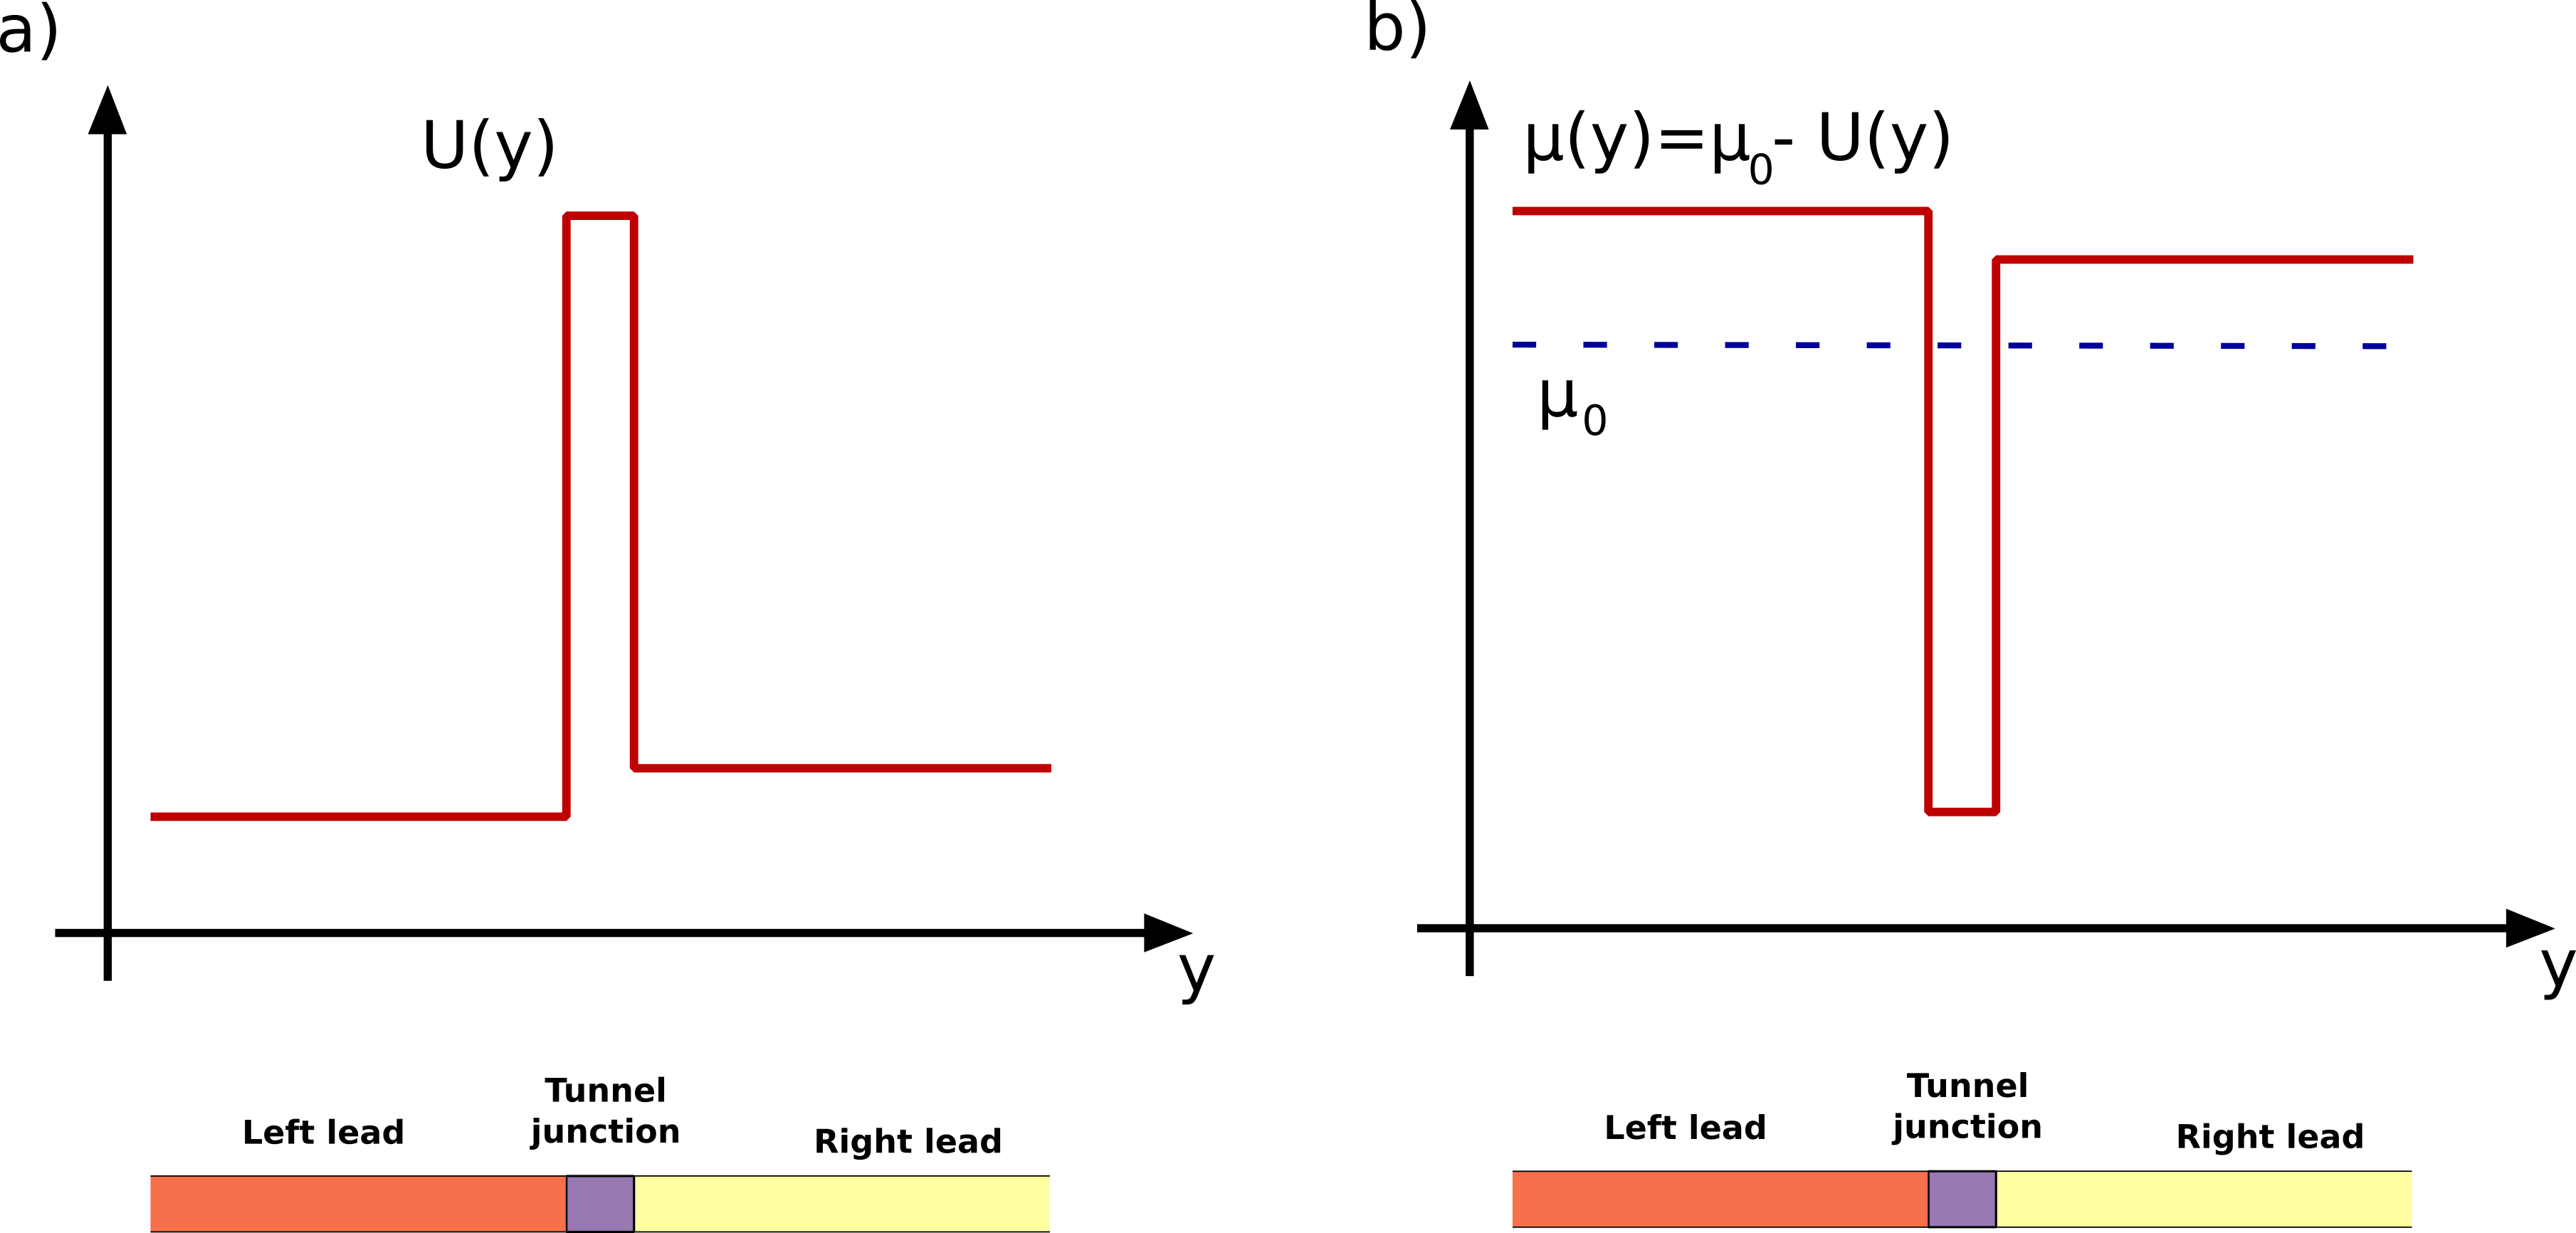
\includegraphics[width=0.8\linewidth]{images/chem_and_ext_potentials}
	\caption{(a) y-profile of external electrical field.  (b) y-profile of effective chemical potential}
	\label{fig:chemandextpotentials}
\end{figure}


Finally, the BdG Hamiltonian for the model reads:
\begin{equation}
\label{full_hamiltonian}
H
=
\br{
	\frac{p^2}{2m}
	-\mu\br{y}
}\tau_z
+
u p \sigma_z \tau_z
+
B\sigma_x	
+
\Delta\br{y}\tau_{\phi\br{y}}
\end{equation}
with
\begin{gather}
\label{full_hamiltonian_suppl}
	\mu\br{y}
	=
	\begin{cases}
		\mu_L,~~~  -\frac{L}{2}<y\\
		\mu_b,~~ -\frac{L}{2} <y <\frac{L}{2}\\
		\mu_R, ~~~~ \frac{L}{2}< y  
	\end{cases}
	~~~~~~~~
	\Delta\br{y}
	=
	\begin{cases}
		\Delta,&~~~  y>\frac{L}{2},~y<-\frac{L}{2}\\
		0,
		&~~ -\frac{L}{2} <y <\frac{L}{2}\\
	\end{cases}
		\\
	\phi\br{y}
	=
	\begin{cases}
	\phi_L,&~~~  -\frac{L}{2}<y\\
	\phi_R, &~~~~ \frac{L}{2}< y 
	\end{cases}
\end{gather}
with $ L $ being the size of the junction. Note, that the parameters $ B $, $ u $, $ \Delta $ and $ m $ are taken to be constant across the system.
 
  This setup is close to one of the models  considered by Oreg et al. in \cite{Oreg_2010} ("\textit{Spatially varying $ \mu $}" section). The difference is in the profile of $ \mu\br{y} $ -- in \cite{Oreg_2010}  there is a step in effective chemical potential, while here this function has a well.  
  
 In \cite{Oreg_2010} it's also shown that the Majorana fermion appears at the interface between areas with different signs of the difference $ B-\sqrt{\mu^2+\Delta^2} $.  As will be shown further, this is also relevant to the  system presented here. Note, that if $ B > \left|\Delta\right| $ this condition can always be satisfied by choosing appropriate $ \mu_L $ and $ \mu_R $. 
 
 When two wires of different sign of $ g $ are assumed in this work, the trivial wire will always be on the left, while the topological wire will always be on the right.

 The model, described by (\ref{full_hamiltonian}) and (\ref{full_hamiltonian_suppl}) possesses a big number of external parameters. Different areas in this parameter space require different approaches and sometimes lead to completely different physics. Here the certain experimentally reasonable constraints are assumed:
  \begin{gather}
 \label{constraints}
 	\mu_L,\mu_R \ll B \approx \Delta \ll mu^2\ll \left|\mu_b\right|
 \end{gather} 

  The experimental justification of this choice is given in chapter \ref{chap:discssion}. From the theoretical point of view the benefit of constraints $ \mu_L,\mu_R \ll B \approx \Delta \ll mu^2 $ is that they make it possible to use  approximate wavefunctions in the wires. The inequality $ mu^2\ll \abs{\mu_b}$ sets the system in the tunneling regime.
  


\section{The dispersion of a homogeneous wire}

Before discussing the properties of the junction it's necessary to consider a dispersion of a homogeneous wire modeled with the Hamiltonian (\ref{bulk_Hamiltonian}). Although this can be done exactly, it's instructive to obtain this dependence step by step, starting with a simpler model and adding terms until the Hamiltonian (\ref{bulk_Hamiltonian}) is restored.

The starting point is the Hamiltonian consisting only of kinetic energy and chemical potential terms: $ H =\frac{ p^2}{2m} - \mu$. It has simple parabolic dispersion presented on fig. \ref{fig:spectrum}(a). When the spin is introduced and spin-orbit coupling term $ up\sigma_z $ is added, the parabola splits in two (fig. \ref{fig:spectrum}(b)), each one corresponding to its own $ z $-projection of the spin. After introducing a magnetic field with $ B\sigma_x $ term, the gap at the intersection opens (fig. \ref{fig:spectrum}(c)). The next step is introducing the BdG formalism, by adding the multiplier $ \tau_z $ everywhere except for magnetic field term:  $ 	H = \br{\frac{p^2}{2m} 	-\mu_0 }\tau_z +u p \sigma_z \tau_z + B\sigma_x	 $. This procedure doubles the spectra in a way that each eigenvector with energy $ E $ obtains a partner eigenvector with energy $ -E $, so two additional  energy branches appear, being a mirror reflection of  initial dispersion. This is presented on fig. \ref{fig:spectrum}(d), with the dashed lines being BdG partners. The last step is adding the superconducting term $ \Delta\tau_\phi $, which opens the gap where dashed and	 solid lines intersect (fig. \ref{fig:spectrum}(e)).

As was mentioned before, the dispersion can be found explicitly. As was pointed out in \cite{Oreg_2010}, it can be done by squaring the Hamiltonian (\ref{bulk_Hamiltonian}) twice and solving a resulting biquadratic equation, leading to:
\begin{equation}
E^2_{1,2}\br{p}
=
B^2
+
\Delta^2
+
\xi_p^2
+
\br{up}^2
\pm	
2\sqrt{
	B^2 \Delta^2
	+
	B^2\xi_p^2
	+
	\br{up}^2\xi_p^2
}
\end{equation}

with $ \xi_p =\frac{p^2}{2m}-\mu$. This dependence, presented on fig. \ref{fig:spectrum}(f), has two positive and two negative branches, as any BdG dispersion with electron-hole symmetry does. In further discussion only positive (	$ E>0 $) branches are considered $  $, if opposite is not mentioned.

\begin{figure}[H]
	\centering
	\includegraphics[width=\linewidth]{images/spectrum}
	\caption{The dispersion of different Hamiltonians:
		 a)  mere kinetic energy and chemical potential: $ H =\frac{ p^2}{2m} - \mu ~~~$
		 b) spin-orbit coupling added: $ 	H = \frac{p^2}{2m}-\mu_0 + u p \sigma_z ~~~$
		 c) magnetic field added: $ 	H = \frac{p^2}{2m} 	-\mu_0  +u p \sigma_z  + B\sigma_x ~~~~~$
		 d) BdG formalism introduced: $ 	H = \br{\frac{p^2}{2m} 	-\mu_0 }\tau_z +u p \sigma_z \tau_z + B\sigma_x	~~~ $
		 e) The complete Hamiltonian of homogeneous wire: $ 	H = \br{\frac{p^2}{2m} 	-\mu_0 }\tau_z +u p \sigma_z \tau_z + B\sigma_x	+ \Delta\tau_\phi $.
		 The parameters of the Hamiltonians for the plotting are: $ B=0.2 $, $ \Delta=0.3 $, $ u=0.9 $, $ m = 1 $, $ \mu = 0.11 $ 
 }
	\label{fig:spectrum}
\end{figure}

If the constrains (\ref{constraints}) are assumed, the lower branch of this spectra has three minima: one of them is at $ p=0 $ exactly, and two others are at $ p = \pm 2mu $ in the leading order. The last two are not very interesting -- the energy gap  there is approximately equal to $ \Delta $, as it should be due to perturbative introduction of superconducting term. On the contrary, the minimum at $ p=0 $, which is given by\cite{Oreg_2010}:
\begin{gather}
	E_2\br{0}=\abs{g},~~~~g = B -\sqrt{\Delta^2+\mu^2}
\end{gather}
is the most important peculiarity of the spectrum. First, as $\mu\ll B \approx \Delta $, it's the true gap of the spectrum as $  \abs{B^2 -\sqrt{\Delta^2+\mu^2}} \approx  \abs{B-\Delta -\frac{\mu^2}{2\Delta}}\ll\Delta$. Second, the  sign of  $ g $ defines whether the wire host a Majorana state. Here it's useful to introduce the terminology: if $ g>0 $ the wire is called topological", otherwise it's called "trivial". In \cite{Oreg_2010} and \cite{Lutchyn_2010} it was derived, that the contact of trivial and topological wire hosts a Majorana state. It can also be shown (see section \ref{subsect:zero_tunnel}), that this state is present at the end of a topological wire and isn't there for a trivial one.

\if 0
As the presence of Majrana state is defined by the sign of $ g_{L,R} $,  the eigenstates of the system which can demonstrate any topological physics are should wave the energies of the order of $ g_{L,R} $. In this work we will reach the energies $ E\sim	\Delta \gg g_{L,R} $ only once -- in subsection \ref{subsec:supercurrent_sim_Delta}, where the stationary supercurrent from the states near $ \Delta $ is estimated. Within all discussion we assume, that the energies of relevant states 
\fi

Note, that when two wires are considered, there are two gaps, $ g_{L,R} = B-\sqrt{\Delta^2+\mu_{L,R}^2} $. When the magnetic field $ B $ is close to $ \Delta $, one can change the signs of $ g_{L,R} $ by changing $ \mu_{L,R} $ respectively. 

For further discussion it's necessary to clarify the place of $ g_{L,R} $ in the parameter hierarchy of the problem. To do so, we introduce $ \beta=B-\Delta $. As $ B \approx \Delta $, we find that $ \beta\ll B,\Delta $. Recalling $ \mu_{L,R}\ll B, \Delta $, one immediately finds that $ g_{L,R}=B-\sqrt{\Delta^2+\mu_{L,R}^2}\approx\beta -\frac{\mu_{L,R}^2}{2\Delta	} \ll B,\Delta$.


\section{Short-wave and long-wave wavefunctions}
\label{sec:high_and_low_modes}

Though the wavefunctions of (\ref{bulk_Hamiltonian}) can be found explicitly, their form is  complicated enough to stall any further analysis. However, with the parameter hierarchy introduced in the previous section the Hamiltonian (\ref{bulk_Hamiltonian}) can be treated perturbatively with the following strategy.

At first step only kinetic and spin-orbit terms are left in the Hamiltonian (\ref{bulk_Hamiltonian}), so 
\begin{gather}
\label{short-long_hamiltonian}
H\approx\br{\frac{p^2}{2m}+up\sigma_z}\tau_z
\end{gather}

  As the presence of the Majorana state depends on sign of $ g_{L,R} $, all the topological physics appears at the energies $ E\sim g \ll mu^2$, so  the energy term can also  be omitted in Schroedinger equation . This leads to a couple of solutions for the momenta: $ p_{\mathrm{short}}\approx\pm2mu $ and $ p_{\mathrm{long}}\approx0 $ with a corresponding wavefunctions --- short-wave and long-wave ones.
  
  Despite the fact that all the omitted terms in (\ref{short-long_hamiltonian}) are indeed smaller than the left ones, it's can't be taken as zero order Hamiltonian --- it's spectrum is ungapped, so all the solutions of Schroedinger equation are running waves and can't form a localized state. To introduce the gap one needs to add a superconductung term to (\ref{short-long_hamiltonian}). For short-wave ($ p\approx2mu $) wavefunctions it's enough and is treated in section \ref{sec:elimintaing_long-wave}.
  
  For long-wave wavefunctions we can't add the superconducting term without adding a magnetic term, as they both significantly alter the momenta, and, consequentially, the wavefunctions. However, for this case the kinetic term, proportional to $ p^2 $, is much smaller than the spin-orbit term  and thus can be omitted. The resulting Hamiltonian is similar to the ones used in \cite{Oreg_2010,Lutchyn_2010} and treated in section \ref{sec:linearized_hamiltonian}. 
  
